\begin{comment}

\section{Paradigmatic Models}
	\subsection[Classical]{Classical Model}

\begin{frame}
	\frametitle{Classical Ising Model}
	
	2D Classical Ising Hamiltonian with size $L$x$L$ and with PBC:
	\begin{columns}
		\begin{column}{0.5\textwidth}
		
		
\begin{figure}[!h]
		\centering
		\begin{tikzpicture}
			\begin{axis} [width=8cm,height=3.2cm,xmax=1, axis lines=middle, 
			enlargelimits,
			xtick={0.5},ytick={0.},xticklabels={$T_c$},yticklabels={$ $}, 
			xlabel=$T$,ylabel=$w$]
				\draw [dashed, line width=0.5pt,gray] (50,-60) -- (50,60);
				\node[text=blue] at (30,7) {\scriptsize{$M>0$}};
				\node[text=blue] at (30,-8) {\scriptsize{$M<0$}};
				\node[text=red] at (70,7) {\scriptsize{$M=0$}};
				\node[text=red] at (70,-8) {\scriptsize{$M=0$}};
				\node[text=red] at (70,-8) {\scriptsize{$M=0$}};
				\addplot [domain=0:0.5, samples=10,smooth,thick,black] {0};
				\filldraw [red] (49,-0.7) rectangle ++(3pt,3pt); %circle (3pt)
			\end{axis}
		\end{tikzpicture}
	\end{figure}			
	
		\end{column}
		\begin{column}{0.5\textwidth}
		
	\begin{align} % \vec
		H_{\rm cl} = - J\,\sum_{\braket{i,\,\,j}}  &
		S_i \cdot  S_j -  w \cdot \sum _i  S_i  \,\,,\\
		Z = \sum _{\{S_i\}} &\, e^{-H/T}  \,\,;
	\end{align}			
	
		\end{column}
	\end{columns}
	
	\bigskip
	
	\alert{\bf Continuous Transition point:} 
	at $w = 0$ and $T_c =  \frac{2}{\ln(1+\sqrt{2})}\,\,(J=1\,\,{\rm fixed})$\\
	$ $\\
	\alert{RG dimensions}:	
	\begin{align}
		w \longrightarrow y_w = 15/8 \qquad 
		T \longrightarrow y_t =  1	\qquad
		{\rm Metropolis \,\,time}\,\,t \longrightarrow z = 2.1667(5) \,\,.\notag
	\end{align}
\end{frame}


	\subsection[Quantum]{Quantum Models}


\begin{frame}
	\frametitle{Quantum Ising Model}
	
	1D Quantum Ising Hamiltonian for a chain of size $L\,$ and PBC 
	($\hat \sigma_{L+1}^{(k)} = \hat \sigma_1^{(k)}$):
	\begin{align}
		\hat H_{\rm Is} = -\sum_{x=1}^{L} \hat \sigma^{(1)}_x \hat
  		\sigma^{(1)}_{x+1} - g\, \sum_{x=1}^L \hat \sigma^{(3)}_x 
  		- w \sum_{x=1}^L \hat \sigma_x^{(1)}\,\,;
	\end{align}
	$\sigma^{(k)} _x$ are the Pauli matrices on the $x^{\rm th}$ site in the
	$k$-axis direction.
	
	\bigskip
	\bigskip
	
	\alert{\bf Continuous Transition point:} 
	at $w = 0$ and $g_c = 1$\\
	\alert{RG dimensions}:	
	$ $\\
	\begin{align}
		w \longrightarrow y_w = 15/8 \quad 
		& r = g-g_c \longrightarrow y_r =  1	\quad
		{\rm  time}\,\,t \longrightarrow z = 1 \\
		&\hat \sigma _x^{(1)} \longrightarrow y_l = d + z - y_h = 1/8\,\,.\notag
	\end{align}
	
\end{frame}
\end{comment}

%\section[Phase Transitions]{Phase transitions and Critical phenomena}

\begin{frame}
\frametitle{Phase transitions and Critical phenomena}
Many systems undergo a phase transition driven by a control parameter whose variation changes the phase of the system.\\
$ $\\
The order parameter assumes different values in each of the two phases and it shows a non-analytic behavior approaching the transition point.\\
$ $\\
We distinguish the transitions in two types:
\begin{itemize}
\item \textbf{\alert{first-order transitions}} (FOT) where in the infinite volume limit the order parameter is discontinuous across the transition point;
\item \textbf{\alert{continuous transitions}} (CT) in which in the same limit a diverging length scale, characterizing the physical correlations, determines the non-analytical behavior of the order parameter.
\end{itemize}
\end{frame}

%%%%%%%%%%%%%%%%%%%%%%%%%%%%%%%%%%%%%%%%%%%%%%%%%%%%%%%%%%%%%%%%%%%%%%%%%%%%%%%%%%%%%%%%%%%%%%%%%%%%


\begin{frame}
\frametitle{Phase transitions and Critical phenomena}
\framesubtitle{Classical Ising model}
\small{
\begin{figure}[!h]
\centering
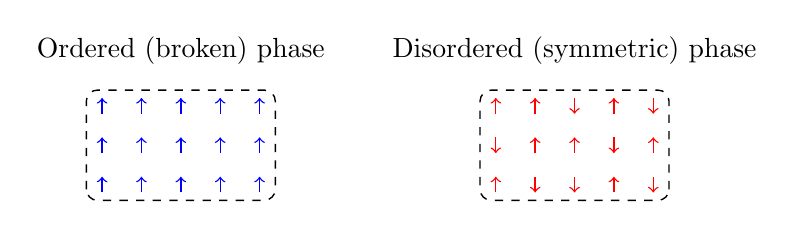
\begin{tikzpicture}
%\draw [dashed, blue, inner color=blue, outer color=white,
%fill opacity=0.4] 
%(0,1) circle (1.5);
%\node[text=blue] (n) at (-1.6,2.5)  {chain};
    \foreach \i in {5,...,9}
    \foreach \j in {1,...,3}
{
\draw [->, line width=0.5pt,blue] (-\i/2,0.2-\j/2) -- (-\i/2,0.4-\j/2);
}

\draw [dashed,line width=0.5pt, black, rounded corners]
        (-4.7,-1.4) rectangle (-2.3,0);
\node at (-3.5,0.5) {\alertb{Ordered (broken) phase}};

\draw [->, line width=0.5pt,red] (1/2,0.2-1/2) -- (1/2,0.4-1/2);
\draw [->, line width=0.5pt,red] (2/2,0.2-1/2) -- (2/2,0.4-1/2);
\draw [<-, line width=0.5pt,red] (3/2,0.2-1/2) -- (3/2,0.4-1/2);
\draw [->, line width=0.5pt,red] (4/2,0.2-1/2) -- (4/2,0.4-1/2);
\draw [<-, line width=0.5pt,red] (5/2,0.2-1/2) -- (5/2,0.4-1/2);
\draw [<-, line width=0.5pt,red] (1/2,0.2-2/2) -- (1/2,0.4-2/2);
\draw [->, line width=0.5pt,red] (2/2,0.2-2/2) -- (2/2,0.4-2/2);
\draw [->, line width=0.5pt,red] (3/2,0.2-2/2) -- (3/2,0.4-2/2);
\draw [<-, line width=0.5pt,red] (4/2,0.2-2/2) -- (4/2,0.4-2/2);
\draw [->, line width=0.5pt,red] (5/2,0.2-2/2) -- (5/2,0.4-2/2);
\draw [->, line width=0.5pt,red] (1/2,0.2-3/2) -- (1/2,0.4-3/2);
\draw [<-, line width=0.5pt,red] (2/2,0.2-3/2) -- (2/2,0.4-3/2);
\draw [<-, line width=0.5pt,red] (3/2,0.2-3/2) -- (3/2,0.4-3/2);
\draw [->, line width=0.5pt,red] (4/2,0.2-3/2) -- (4/2,0.4-3/2);
\draw [<-, line width=0.5pt,red] (5/2,0.2-3/2) -- (5/2,0.4-3/2);

\draw [dashed,line width=0.5pt, black, rounded corners]
        (2.7,-1.4) rectangle (0.3,0);
\node at (1.5,0.5) {\alert{Disordered (symmetric) phase}};

%       \filldraw [red] (0,0) rectangle ++(6pt,6pt); %circle (3pt);
%        \draw[thick,<->,gray] (0,-0.3)--(0,-0.8);
%        \draw [dashed,thick, black, rounded corners]
%        (-0.35,-1.8) rectangle (0+0.35,-0.9);
%        \filldraw[red!50!white, rounded corners]
%        (-0.35,-1.8) rectangle (0+0.35,-0.9);
%        \node at (0,-1.35) {$\mathcal{B}$};
\end{tikzpicture}
\end{figure}}
As example, we take the classical Ising model in which:
\begin{eqnarray} % \vec
&H = - J\,\sum_{\braket{i,\,\,j}}  S_i \cdot  S_j -  h \cdot \sum _i  S_i & \,\,,\\
&Z = \sum _{\{S_i\}} \, e^{-H/T} & \,\, ,
\end{eqnarray}
%where $\vec S_i$ is a d-dimensional vector with $\vec S_i \cdot \vec S_i = 1\,$. 
where $ S_i = \pm 1\,$ and $i,\,j$ indicate the sites of a $d$-dimensional lattice. 
%The system undergoes a CT driven by the temperature $T\,$ and described by the order parameter \alertb{$M=V^{-1}\sum _i  \braket{S_i}\,$} for $V\to +\infty\,$. 
\small{
\begin{figure}[!b]
\centering
\begin{tikzpicture}
\begin{axis} [width=8cm,height=3.2cm,xmax=1, axis lines=middle, enlargelimits,
xtick={0.5},ytick={0.},xticklabels={$T_c$},yticklabels={$ $}, xlabel=$T$,ylabel=$h$]
\draw [dashed, line width=0.5pt,gray] (50,-60) -- (50,60);
\node[text=blue] at (30,7) {\scriptsize{$M>0$}};
\node[text=blue] at (30,-8) {\scriptsize{$M<0$}};
\node[text=red] at (70,7) {\scriptsize{$M=0$}};
\node[text=red] at (70,-8) {\scriptsize{$M=0$}};
\node[text=red] at (70,-8) {\scriptsize{$M=0$}};
\addplot [domain=0:0.5,
samples=10,smooth,thick,black]
{0};
\filldraw [red] (49,-0.7) rectangle ++(3pt,3pt); %circle (3pt)
\end{axis}
\end{tikzpicture}
\end{figure}
}

\end{frame}


% With the characteristic length scale equal to infinity, we may guess that the structure of the correlations is the same at all length scales, i.e. the physics is invariant under a scaling transformation.

%%%%%%%%%%%%%%%%%%%%%%%%%%%%%%%%%%%%%%%%%%%%%%%%%%%%%%%%%%%%%%%%%%%%%%%%%%%%%%%%%%%%%%%%%%%%%%%%%%%%

\begin{frame}
\frametitle{Phase transitions and Critical phenomena}
\framesubtitle{Power-laws}
The CTs are characterized by power-law behavior:\\
$ $\\
\begin{itemize}
\item the correlation length $\xi$ defined as 
\[
\lim_{\abs*{i-j}\to \infty}\braket{ S_i \cdot S_j}\sim e^{-\abs*{i-j}/\xi}\,,
\]
scales as $\alertb{\quad \xi \sim \abs*{t}^{-\nu}}\,\,, \quad t = T/T_c -1 \,$;
\item the order parameter $M\,$: $\quad \alertb{ M \sim \abs*{t}^\beta}\,$;
\item the susceptibility $\chi = \sum _i \braket{ S_i \cdot S_j} \,$: $\quad \alertb{ \chi \sim \abs*{t}^{-\gamma}}\,$;
\end{itemize}
$ $\\
where the parameters $\nu\,,\,\,\beta\,,$ and $\gamma$ are called critical exponents.\\ 
$ $\\
%Since $\nu = 1$ for $d=2\,$, close to $T=T_c$ the correlation length diverges to $\infty\,$.
Close to the critical point, i.e. $t \to 0\,$, the correlation length diverges to $\infty\,$.
\end{frame}

%%%%%%%%%%%%%%%%%%%%%%%%%%%%%%%%%%%%%%%%%%%%%%%%%%%%%%%%%%%%%%%%%%%%%%%%%%%%%%%%%%%%%%%%%%%%%%%%%%%%

\begin{frame}
\frametitle{Phase transitions and Critical phenomena}
\framesubtitle{Renormalization group (RG)}

% With the characteristic length scale equal to infinity, we may guess that the structure of the correlations is the same at all length scales, i.e. the physics is invariant under a scaling transformation under which the coordinates change as $$$x → x = x/b, (4.1)$$$ where b is the rescaling factor. In other words, the basic structure of all correlations should be invariant under a transformation from the x to the x' coordinates. An example of this invariance appears in our result for the two-point correlation function C(x) ∼ x^{2−D} for x << ξ .

Close to critical point, the many-body system shows an universal critical behavior dependent only by few global properties:
\begin{itemize}
\item \alert{the space dimensionality $d\,$},
\item \alert{the nature and the symmetry of the order parameter},
\item \alert{symmetry-breaking pattern}.
\end{itemize}
$ $\\
$ $\\
These features are encoded in the \alertb{renormalization group (RG) theory} in which:
\begin{itemize}
\item we have a RG flow in the Hamiltonian space,
\item the critical points are described by the fixed points of the theory,
\item only a few perturbations are relevant, the corresponding positive eigenvalues are related to the critical exponents.
\end{itemize}
\end{frame}

%%%%%%%%%%%%%%%%%%%%%%%%%%%%%%%%%%%%%%%%%%%%%%%%%%%%%%%%%%%%%%%%%%%%%%%%%%%%%%%%%%%%%%%%%%%%%%%%%%%%

\subsection{Quantum transitions}

\begin{frame}
\frametitle{Quantum Transitions}
%\framesubtitle{Lindblad equation}
\textbf{\alertb{Quantum phase transitions}} are driven by the variation of the Hamiltonian parameters which determine the non-analytic behavior of the ground state.\\
$ $\\
In the large-volume limit, the \alertb{continuous quantum transitions} (CQT) are characterized by:
\begin{itemize}
\item a diverging correlation length: 
\begin{equation}
\alert{\xi \sim \abs*{\bar g}^{-\nu}} \,\,;
\end{equation}
\item a lowest energy gap $\Delta$ which vanishes:%qtime associated with a classic length l_c, so \xi_c \to \Delta
\begin{equation}
\alert{\Delta \sim \xi^{-z} \sim \abs*{\bar g}^{z\,\nu}} \,\,;
\end{equation}
\end{itemize}
where $\bar g = g - g_c$ is an Hamiltonian parameter which drives the quantum transition and $z$ is the dynamic critical exponent.
\end{frame}

\begin{frame}
	\frametitle{Quantum Transitions}
	\framesubtitle{Example - Quantum Ising model}
	
	As a paradigmatic model for quantum transitions, we consider the quantum Ising model whose Hamiltonian is given by:
	\begin{equation}
	\alert{
	  \hat H_{\rm Is} = -\sum_{x=1}^{L-1} \hat \sigma^{(1)}_x \hat
	  \sigma^{(1)}_{x+1} - g\, \sum_{x=1}^L \hat \sigma^{(3)}_x }\,\,,
	  \label{ising}
	\end{equation}
	where $\sigma^{(j)} _x$ are the Pauli matrices on the $x^{\rm th}$ site of the chain and $L$ is the system size.\\
	$ $\\
	
	The system undergoes a \alert{quantum transitions} at $\alert{g_c=1}\,$, between paramagnetic and ordered phases.\\
\end{frame}



%\section{Kitaev model}
\begin{frame}
	\frametitle{Kitaev Model}
	Kitaev Hamiltonian mapped into a spin-$1/2$ XY chain, by a 
	Jordan-Wigner transformation (OBC):
	$\qquad \qquad\alert{\hat c \longrightarrow \hat\sigma}\,$
	\begin{align}
		\label{KitaevH}
		\hat H _K^{\rm (ABC)} =- \sum _{x=1}^{L}\biggr[ \bigl(
		 \hat c_x^\dagger \, \hat c_{x+1} + 
		 \hat c_{x+1}^\dagger \,\hat c_x \bigl) + 
		 \delta\,\bigl( \hat c_x \, \hat c_{x+1} + 
		\hat c_{x+1}^\dagger \, \hat c_x^\dagger \bigl)\biggr] - 
		\sum _{x=1}^L  \mu \, \hat c_x^\dagger \, \hat c_{x}  \,\,;
	\end{align}
	\begin{figure}[!h]
		\centering
		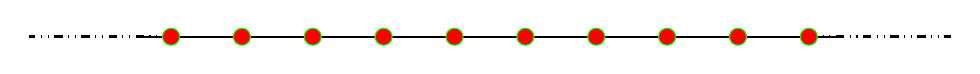
\begin{tikzpicture}[scale=0.9]
			\draw [-, line width=0.8pt, black] (-5.5,0.5) -- (4.5,0.5);

			\draw [dash dot dot, line width=1.2pt, black] (-5,0.5) -- (-7,0.5);
			\draw [dash dot dot, line width=1.2pt, black] (4,0.5) -- (6,0.5);

			\fill [red, draw=green] (-5,0.5) circle (0.12);
			\fill [red, draw=green] (-4,0.5) circle (0.12);
			\fill [red, draw=green] (-3,0.5) circle (0.12);
			\fill [red, draw=green] (-2,0.5) circle (0.12);
			\fill [red, draw=green] (-1,0.5) circle (0.12);
			\fill [red, draw=green] (4,0.5) circle (0.12);
			\fill [red, draw=green] (3,0.5) circle (0.12);
			\fill [red, draw=green] (2,0.5) circle (0.12);
			\fill [red, draw=green] (1,0.5) circle (0.12);
			\fill [red, draw=green] (0,0.5) circle (0.12);
			%\node (n) at (-4.5,0.85)  {$\bm{\hat c_1} $};
			%\node (n) at (4.5,0.95)  {$\bm{\hat c_L^\dagger} $};
		\end{tikzpicture}
	\end{figure}

	\alert{\bf Continuous Transition point:} 
	\begin{align}
		\mu _c = -2 \qquad {\rm and} \qquad \delta = 1 \,\,{\rm fixed} \,\,;\notag
	\end{align}
	\alert{RG dimensions}:	
	$ $\\
	\begin{align}
		w = \mu - \mu_c \longrightarrow y_w = 1 \qquad 
		\hat c_x \, ,\,\, \hat c_x^\dagger \longrightarrow y_c = 1/2 \qquad
		{\rm dynamic \,\, exp:\,\,} z =1
		\,\,.\notag
	\end{align}
	
\end{frame}


\subsection[FSS]{Finite Size Scaling (FSS) at the equilibrium}

\begin{frame}
\frametitle{Finite Size Scaling (FSS) at the equilibrium}
\framesubtitle{Kitaev model}
\small
At the critical point, the \alert{ground state} $\ket{0}\bra{0}$ correlation function:
\begin{equation}
%\begin{subequations}
\label{correlations}
%\begin{align}
\alertb{
G_c(x,y,t)}  \alertb{ =  
\braket{0 \big| \hat c_{x}^\dagger \hat
  c_{y}^{\phantom\dagger} + \hat c_{y}^\dagger \hat
  c_{x}^{\phantom\dagger} \big| 0}}\,\,,%\label{ctf}
%\alertb{G_p(x,y,t)} & \alertb{= {\rm
%  Tr}[\rho(t) (\hat c_{x}^\dagger \hat c_{y}^\dagger + \hat
%  c_{y}^{\phantom\dagger} \hat c_{x}^{\phantom\dagger})]}\,\,.
%\end{align}
%\end{subequations}
\end{equation}
satisfies for $L\to \infty\,$ and using RG theory:
\begin{equation}
\alert{
G_{c}(x,y,\bar \mu)= b^{-2y_c} \,\mathscr{G}_{c} \left( x/b, y/b, \bar \mu \,b^{y_\mu}\right)} \,\,,
\end{equation}
where $y_\mu=1\,,\,\,y_c=1/2$ are the RG dimensions of, respectively, the parameter $\mu$ and the fermionic operator $\hat c_x$ and $\hat c_x^\dagger\,$.\\
$ $\\
$ $\\
$ $\\
If the system size $L$ is finite \alert{$\Longrightarrow$} in the FSS limit, i.e. when we keep the ratio \alertb{$\xi / L\,$} fixed for $L \to \infty$; in other words, when wee fix \alertb{$b=L$}, we have:
\begin{eqnarray}  
\label{scalKitaev}
\alert{
G_{c}(x,y,\bar \mu; L)= L^{-1} \,\Bigr[\mathscr{G}_{c} \left( X, Y, \kappa\right) + O(L^{-1}) \Bigr]} \,\,,\\
\alertb{X \equiv x/L}\,, \qquad \alertb{Y \equiv y/L}\,, \qquad \alertb{\kappa = \bar \mu \,L^{y_\mu} }\,\,.
\end{eqnarray}

\end{frame}
